\chapter{Введение}


В последние годны наблюдается заметный рост количества уязвимостей в программном обеспечении. Так, согласно статистике \cite{CVEstats}, в $2016$ году было обнаружено $6447$ уязвимостей, в $2017$ --  $14714$, a в $2018$ -- $16555$. Это связано как с объемом и сложностью, разрабатываемого программного обеспечения, так и с развитием техник тестирования безопасности.

\begin{figure}[h]
    \center{
        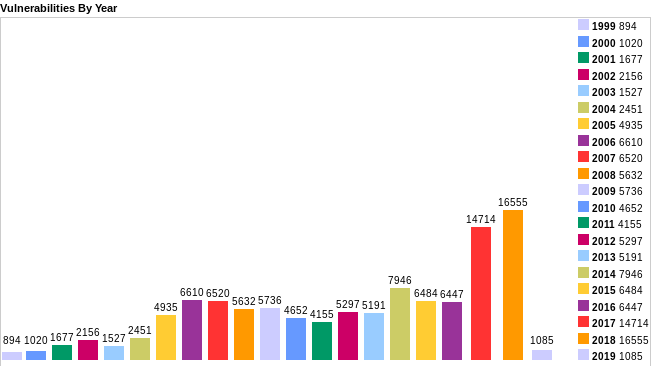
\includegraphics[scale=0.5]{img/cve_stats.png}
    }
    \caption{Cтатистика опубликованных уязвимостей за последние 20 лет}
    \label{fig:image}
\end{figure}

Одним из популярных подходов к автоматизации поиска уязвимостей является фаззинг-тестирование. Это
техника тестирования программного обеспечения, заключающая в автоматической генерации входных данных. Целью фаззинга является нахождение таких входных данных, которые вызовут аварийное завершение программы.

Для достижения своей цели фаззеру необходимо генерировать входные данные, позволяющие пройти по разным путям выполнения. Один из популярных подходов, впервые примененный в AFL \cite{AFL} заключается в мутировании изначальных входных данных с целью увеличения покрытия.

Несмотря на высокую эффективность такого подхода он не лишен недостатков. Так например для кода
\begin{lstlisting}[environoment=C_LANG, label=example1]
uint32_t buf[10];
read(10, &buf, 40);
buf[0] &= 500;

if (buf[0] == 100) {
    //branch 1
    ...
} else {
    //branch 2
    ...
}
\end{lstlisting}

для того, чтобы найти входные данные для прохождения по ветке $1$ необходимо фактически перебрать $2^32$ значений. Для решения подобных проблем в \cite{DRILLER} предлагается подход, основанный на динамическом символьном выполнении. В случае если фаззер не может сгенерировать входные данные для прохождения по некоторой ветки в течение некоторого ограниченного времени, запускается модуль символьного выполнения, который составляет и решает предикат пути. Затем фаззер продолжает свою работу.
Подход из \cite{DRILLER} реализован в инструменте \emph{DRILLER}, распространяемом под открытой лицензией.

Комбинирование фаззинга и символьного выполнения тоже имеет свои сложности:
\begin{itemize}
    \item Генерация формул для каждой инструкции достаточно времязатратная операция.
    \item Задача поиска решений символьных уравнений является \textbf{NP полной}, не смотря на наличие множества эвристик невозможно гарантировать решение предиката пути за разумное время.
\end{itemize}

В данной работе предлагается иной способ улучшения эффективности открытия фаззером новых путей. Так в \ref{example1} фаззер не знает от каких входных данных зависит условный переход и может мутировать все байты входного файлв для открытия ветки $1$, однако в действительности значение \textbf{buff[0]} определяется только одним байтом, и только его и имеет смысл мутировать.
Так если у фаззера будет возможность для каждого условного перехода узнать от каких входных данных зависит его выполнение, это позволит существенно сократить количество итераций, необходимых для открытия пути.

Предметом работы является исследование и разработка методов, позволяющих предоставить фаззеру искомую информацию.



\chapter{Обзор}

% \chapter{Методы реализации динамического анализа}

\section{Динамический Анализ}

Динамический анализ - это анализ, заключающийся в непосредственном выполнении кода. Однако, просто запустить программу может быть недостаточно. Существует несколько способов получения дополнительной информации во время выполнения:

\begin{itemize}
\item {\em Исполнение кода в виртуальном окружении}. При данном подходе программа запускается внутри некоторого программного эмулятора. Например qemu \cite{QEMU}.
%\item $\sigma$ is a {\em symbolic store} that associates program variables with expressions over \mynote{[D] $\alpha_i$ also concrete?} concrete and symbolic values $\alpha_i$.

\item {\em Статическая инструментация}.
Статическая инструментация бывает двух видов.
    \begin{itemize}
        \item {\em Статическая инструментация исходного кода}. В случае, если имеется доступ к исходному коду, можно просто внести изменения в текстовые файлы с кодом. Добавление отладочной печати может быть примером статической инструментации исходного кода. Подобный вид инструментации также поддерживается непосредственно компилятором. Так GCC имеет опцию  \textit{-finstrument-functions}
        \item {\em Статическая инструментация бинарного кода (SBI)}. В случае отсутствия исходного кода, изменениям может быть подвержен сам исполняемый файл на диске. Тривиальным примером такой инструментации может быть например замена условных переходов на \textint{nop} инструкции. 
    \end{itemize}

\item {\em Динамическая бинарная инструментация}. Данный вид инструментации позволяет вносить изменения в программу непосредственно в процессе её выполнения. Подробное описание возможных подходов к реализации динамической инструментации можно найти в \cite{PBA}.
\end{itemize}

В данной работе проводилось исследование инструментов, основанных на использовании эмуляторов и динамической бинарной инструментации.


\section{Динамическая бинарная инструментация}

Основная идея динамической инструментации заключается в том, что инструментирующая программа контролирует все выполняемые инструкции. Классическая реализация работает примерно следующим образом. Перед непосредственным запуском программы происходин настройка модуля динамической инструментации и устанавливаются функции обратного вызова для различных видов событий, затем код инструментируемой программой считывается по базовым блокам и выполняется.

Рассмотрим несколько популярных DBI инструментов.

\subsection{QDBI}

В \cite{QDBI} \emph{QDBI} - расшифровфывается как \emph{QuarkslaB Dynamic binary Instrumentation}, авторы позиционируют его как кросплатформенный и кроссархитектурный фреймворк динамической бинарной инструментации. В планах разработчиков поддержка операционных систем Linux, macOS, Android, iOS и Windows, а также архитектур  x86, x86-64, ARM и AArch64.

Однако, в настоящий момент полноценно поддерживаются только Linux, macOS, Windows на x86-64 архитектуре, при этом поддержки SIMD инструкций нет.

Cогласно \cite{QDBI} архитектура \emph{QDBI} описывается следующей схемой.
\begin{figure}[H]
    \center{
        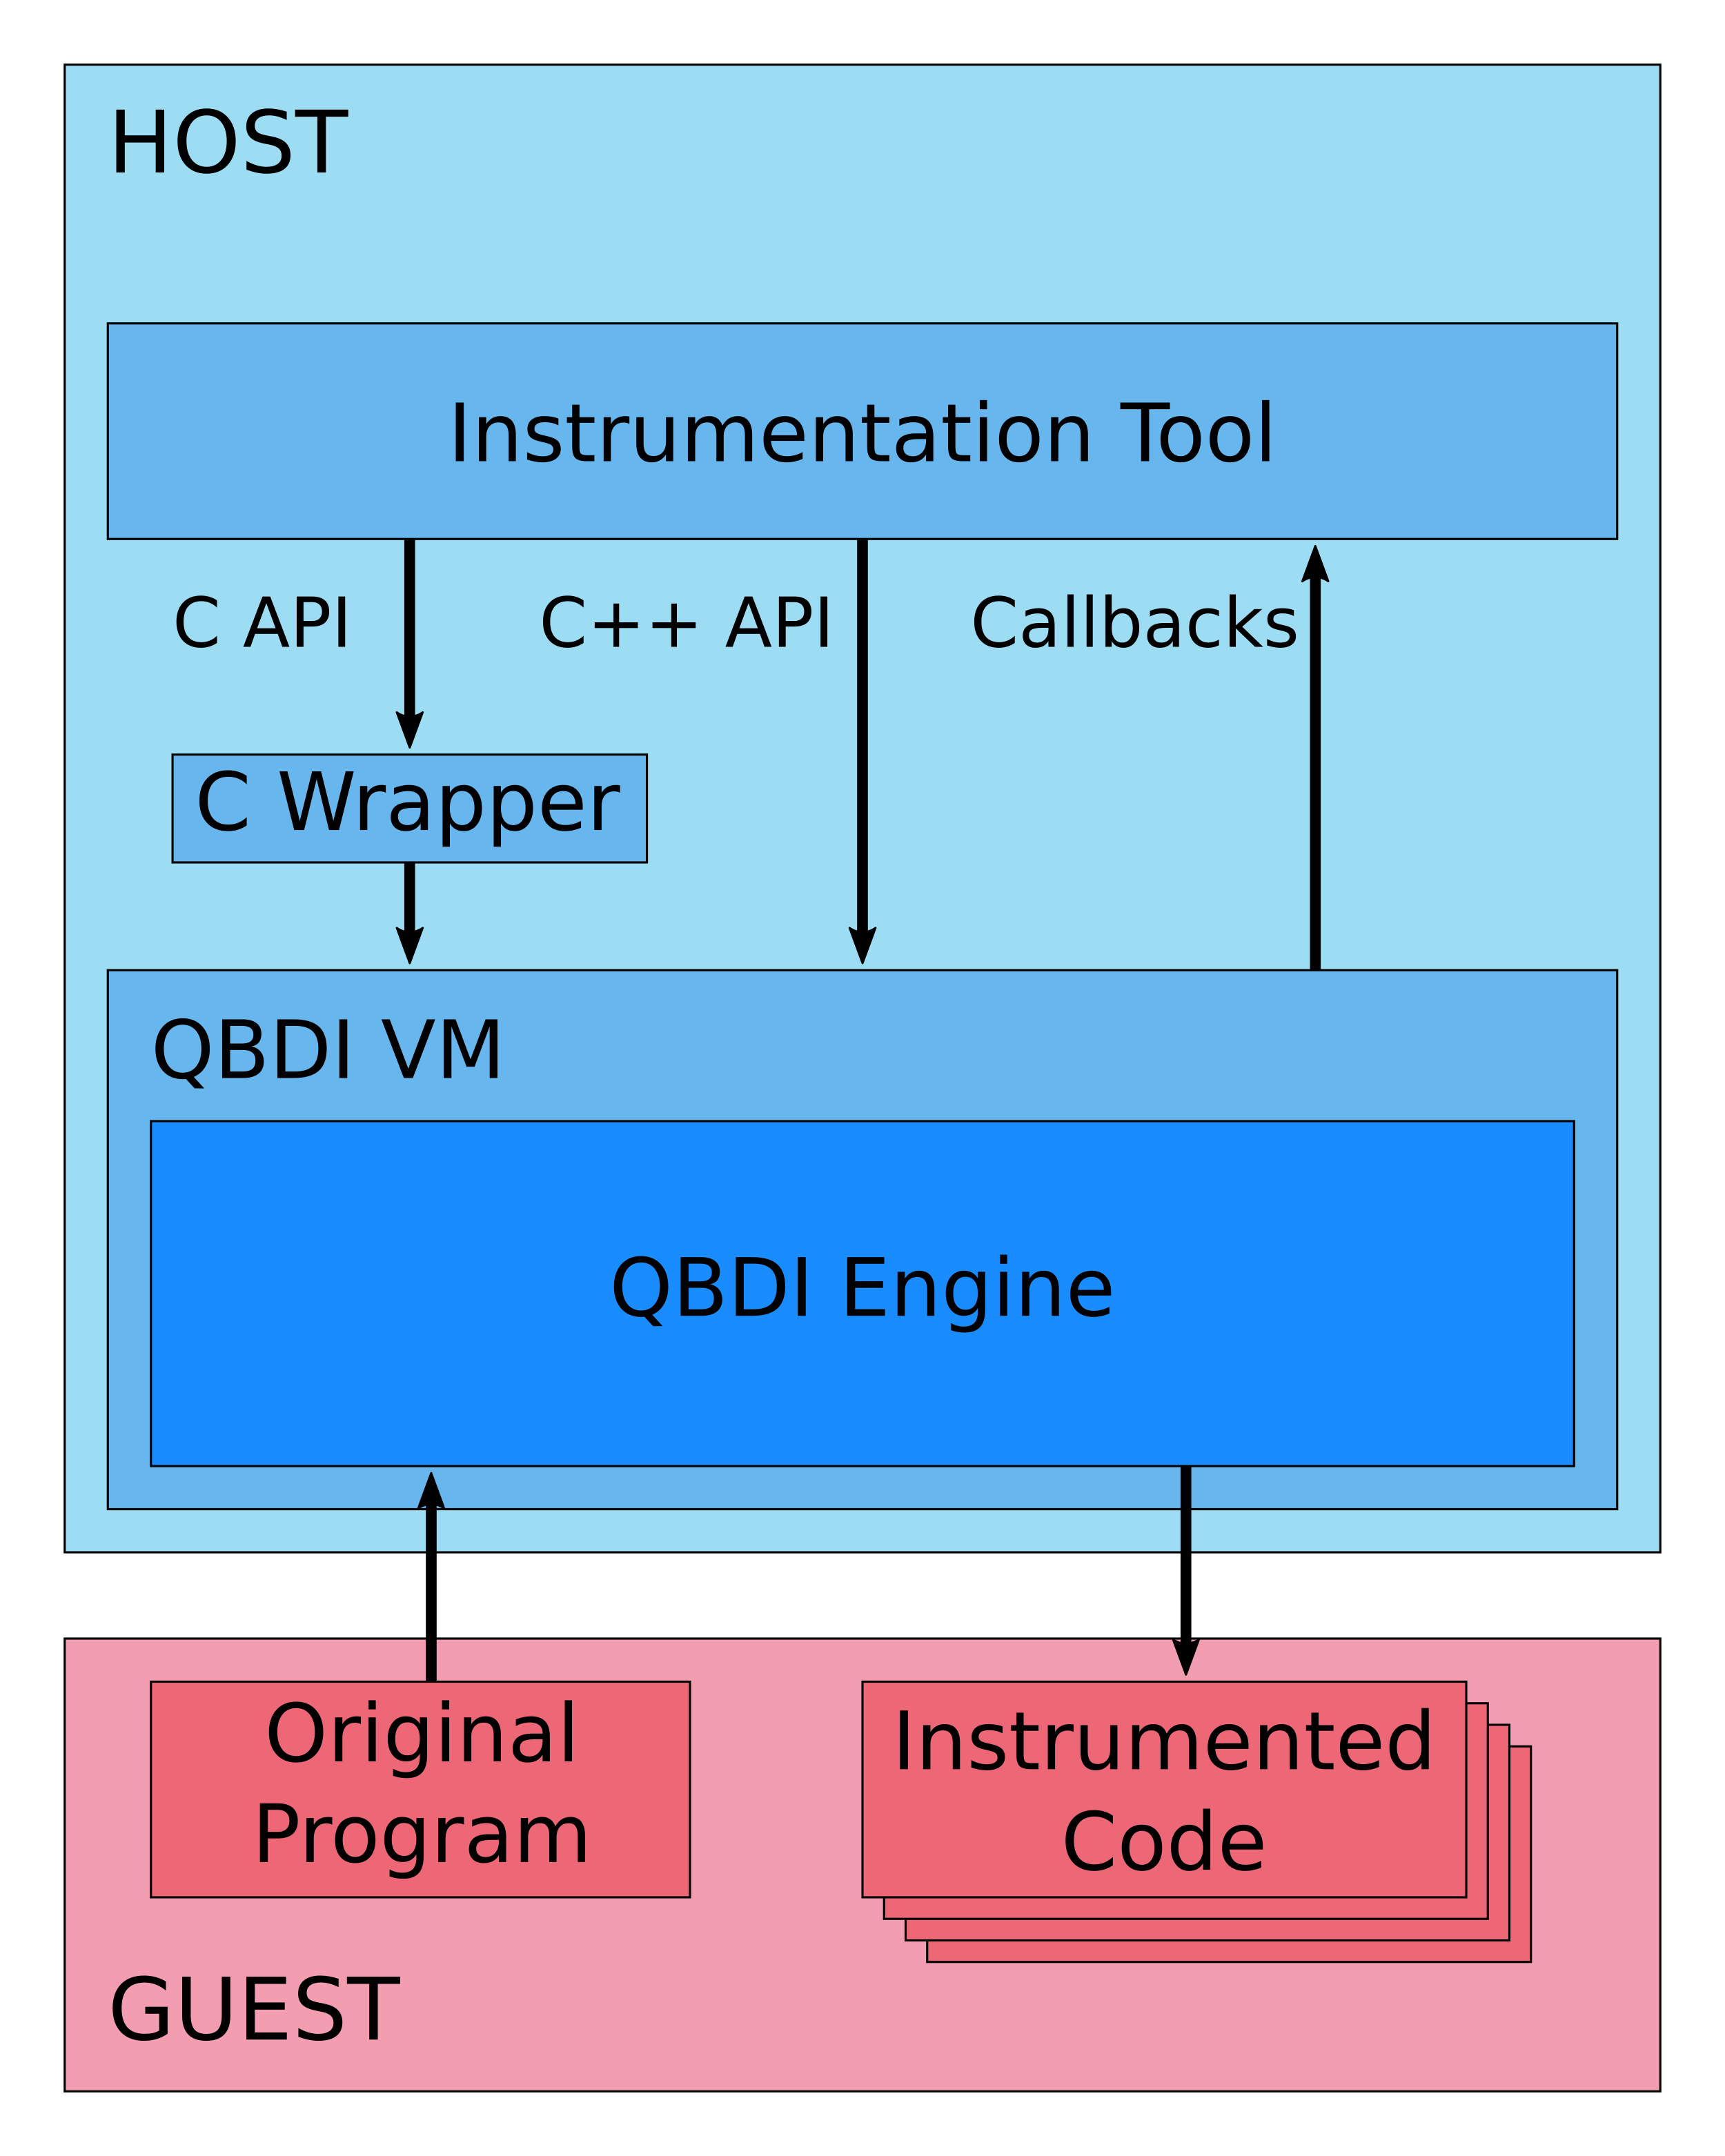
\includegraphics[scale=0.5]{img/qdbi_architecture.png}
    }
    \caption{Архитектура QDBI}
    \label{fig:qdbi}
\end{figure}

В качества хоста выступает пользовательская программа инструментации, написанная с использованием QDBI API, которое позволяет установить функции обратного вызова для различных событий.

\emph{QDBI} представляет из себя модуль, управляющий выполнением оригинальной программы. Он считывает в цикле код следующего базового блока, а затем при помощи JIT генерирует его пропатченную версию вместе с кодом инструментации. Все это происходит в одном адрессном пространстве, что ограничивает возможности QDBI. В частности он не позволяет инструментировать код загрузчика.

QDBI может использоваться двумя принципильно различными способами. В первом случае предполагается наличие исходного кода. В таком случае есть возможность проводить анализ не только программы целиком, но и отдельных функций, предварительно сформировав окружение. При этом фактически производится статическая инструментация исходного кода вручную.

Другой вариант работы более универсален. Инструментирующая программа пишется как отдельной приложение, а фактическая инструментация происходит посредством добавления QDBI библиотеки в LD\_PRELOAD.

Поскольку QDBI является достаточно молодой технологией, в настоящий момент известных инструментов основанных на нем не существует.


\subsection{Valgrind}

\emph{Valgrind} это доcтаточно необычный фреймворк динамической бинарной инструментации. Был разработан Николасам Нетеркот в рамках его работы над PHD диссертацией. Хорошее описание фреймворка его особенностей и устройства можно найти в \cite{VALGRIND}.


\emph{Valgrind} лелится на ядро и модули, где собственно ядро предоставляет возможности для бинарной инструментации, а модули представляют собой конкретные инструменты с некоторым функционалом, работаюшие с API ядра. Одним из наиболее популярных модулей является \emph{memcheck} - инструмент для поиска утечек памяти.

Ядро \emph{Valgrind} считывает инструкции инструментируемого приложения и транслирует их в промежуточный язык (IL), VEX. Трансляция производится по базовым блокам, для оттранслированного базового блока вызывается функция инструментации запущенного модуля, после чего ядром производится JIT компиляция и выполнение полученного кода.

\emph{Valgrind} поддерживает следующие платформы.

\begin{itemize}

    \item x86/Linux: Отсутсвует поддержка SSE4, AVX, AVX2 инструкций.
    \item AMD64/Linux: Поддерживаются все инструкции, включая AVX2.
    \item PPC32/Linux, PPC64/Linux, PPC64LE/Linux
    \item S390X/Linux: supported
    \item ARM/Linux: Поддерживается начиная с ARMv7.
    \item ARM64/Linux: Поддерживается начиная с ARMv8.
    \item MIPS32/Linux, MIPS64/Linux
    \item X86/Solaris, AMD64/Solaris, X86/illumos, AMD64/illumos: Поддержка начиная с Solaris 11.
    \item X86/Darwin (10.10, 10.11), AMD64/Darwin (10.10, 10.11)
    \item ARM/Android, ARM64/Android, MIPS32/Android, X86/Android:
\end{itemize}

\emph{x86/FreeBSD}, \emph{x86/NetBSD} и \emph{sparc64/Linux} поддерживаются сторонними разработчиками.

Как и \emph{QDBI}, \emph{Valgrind} работает в одном вдресном пространстве с инструментируемым приложением. Кроме того, поскольку загрузка осуществляется самим \emph{Valgrind} модули должны быть собраны без использования динамических библиотек.

\subsection{Pin}

Pin - это свободно распространяемый фреймворк для динамической бинарной инструментации с закрытым исходным кодом, подробно прочитать о его устройстве можно в \cite{PIN} или \cite{PBA}.

Pin поддерживает x86 и amd64 архитектуры и работает на операционных системах Linux, Windows и macOS. Pin принимает на вход исполняемый файл и последовательно считывает из него инструкции, затем при необходимости инструментирует их, компилирует при помощи JIT компиялотора и выполняет.

Инструменты написанные на основе Pin называются pintools. Pin предоставляет API основанный на функциях обратного вызова. При этом концептуально инструментация в pin состоит из двух частей

\begin{itemize}
    \item Принятие рещения какой код куда следует вставить. (\emph{Инструментирующий код})
    \item Пользовательский код, вставляемый в точках, определенных в прошлом пункте (\emph{Анализирующий код})
\end{itemize}

Соответсвенно к инструментирующему коду относится код, отвечающий за установку функций обратного вызова при наступлении некоторых событий, а к анализирующему коду относятся непосредвенно функции обратного вызова.

Выгодно отличает Pin от расмотренных ранее инструментов бинарной инструментации достаточно богатое API, предоставляющее большее количество событий, на которые можно установить свои обработчики. В частности, вместе с Pin поставляется дизассемблер \emph{Xed}, благодаря которому есть возможность программно извлекать информацию о семантике инструкций.

Pin поддерживает разные уровни гранулярности для инструментации, так можно поставить свой обработчки на всю трассу выполнения, на базовый блок, или на конкретную инструкцию. При этом следует учитывать, что базовый блок с точки зрения Pin может не быть таким на самом деле, поскольку нет возможности определить существуют ли переходы в середину предполагаемого базового блока.

Pin позволяет также инструментировать процесс загрузки кода, вызывая обработчики на загрузку динамических библиотек.

Следует отметить, что для версии Pin $2.14$ не гарантируется корректная работа на версиях ядра Linux 4 и старше, с другой стороны новые версии Pin используют \emph{Pin Crt} вместо системных библиотек, что накладывает определенные ограничения на pintools:

\begin{itemize}
    \item Реализация стандартной библиотека с++ не поддерживает возможности стандартов с++11 и новее.
    \item При желании произвести линковку с внещней библиотекой, необходимо чтобы эта библиотека была собрана с PinCrt вместо системной библиотеки.
\end{itemize}

\section{Анализ помеченных данных}

Динамический анализ помеченных данных (Dynamic Taint Analysis, DTA), также известный как динамический анализ потока данных (Dynamic Flow tracking, DFT) - это техника анализа програм, позволяющая определить какие состояния программы зависят от входных данных.
% Существует также статический анализ потока данных

Примером классической задачи, решаемой при помощи анализа помеченных данных, может служить задача определения достигают ли данные из недоверенного источника "Опасных" функций. Многие уязвимости в программном обеспечении обусловлены недостаточным контролем над входными данным. Применение анализа потока данных позволяет детектировать подобные проблемы.

Динамический анализ помеченных данных делится на 3 фазы

    \begin{itemize}
        \item {\em Определение источников помеченных данных}. На данном этапе определяется каким данные должны быть помечены. Обычно метками снабжаются данные, получаемые из недоверенного
        источника. В зависимости от типа приложения, это могут быть данные полученные по сети, из файла, или потока стандартного ввода.
        \item {\em Распространение пометок (Taint propogation)}. Для отслеживания потока данных, 
        для каждой инструкции манипулирующей данными необходимо написать инструментирующий код для манипуляции метками. Так, например инструкция \textint{mov eax, ebx} перезаписывает метку для регистра eax меткой регистра \textint{ebx}. Это фаза является самой сложной, поскольку оставляет много открытых вопросов. К примеру
        \begin{itemize}
            \item Следует ли отслеживать помеченность побайтово или побитово? Если \textint{eax} помечен, то после команды \textint{or eax, 0x746567bc} контролируются уже не все биты. Однако, в большинстве случаев отслеживание каждого бита может быть слишком дорогой операцией.
            \item Следует ли помечать адрес памяти, на который указывает помеченная переменная?
            \item Если условный переход зависит от помеченных данных, следует ли считать что последующие инструкции тоже от них зависят?
            \item Как хранить информацию о помеченных адресах в памяти?
            \item Cледует ли различать пометки, полученные из разных источников?
        \end{itemize}
        \item {\em Применение политик безопасности}. Фаза, на которой используются результаты анализа. Происходящее на этом этапе зависит от изначальных целей анализа. Типичным примером может быть отслеживание попадания помеченных данных в аргументы некоторых заранее выделенных функций, или факта помеченности счетчика инструкций.
    \end{itemize}


% \section{методы реализации технологии анализа помеченных данных}
% Рассмотрим несколько подходов к реализации анализа помеченных данных.

% % \subsection{Символьное выполнение}

% \subsection{Множество помеченных адресов}

% \subsection{Хэш таблица с побайтовыми метками}

% \section{Теневая память для хранения информации о пометках}


% \section{Обзор технологий анализа помеченных данных}


\subsection{Triton}

\subsection{Taintgrind}

\subsection{Moflow gentrace}

\subsection{libdft}

\section{Динамическое символьное выполнение}


\subsection{Triton}

\subsection{angr}

\subsection{manticore}



% \chapter{Сравнение инструментов для динамического анализа}

% \section{Библиотека для снятия и анализа трас}

% \section{Результаты сравнение}

% \section{Выводы}




\chapter{Методы определения входных данных влияющих на условные переходы}

% Для начала расмотрим самый простой способ

\section{Использование символьного выполнение}

\subsection{Решение на основе Angr}


\section{Использование меток помеченных данных}

\section{Комбинированный подход}

Оба предыдыщих подхода имеют недостатки. Построение символьных формул для всех инструкций может быть достаточно ресурсоемкой задачей. Время работы \em{Triton} может быть тому примером. В случае же, если используется онлайн символьное выполнение - проблема стоит еще острее, так \em{angr} вообще оказывается не очень применим на программах размером больше чем задания для CTF соревнований.
\\
С другой стороны, многие технологии анализа помеченных данных не поддерживают гранулярность на уровне отдельных байт, и возможность отследить от каких именно входных байт зависит некоторый адрес или регистр отсутствует. Даже если есть возможность отследить метки на каждый байт, существуют примеры когда этого недостаточно. так в \cite{Cavallaro07anti-taint-analysis:practical} приводится следующий пример, где между x и y есть взаимно-однозначное соответствие, которое не отслеживается динамическим анализом помеченных данных.
\\

\begin{lstlisting}[environoment=C_LANG]
char y[256], x[256];
...
int n = read(network, y, sizeof(y));
for (int i=0; i < n; i++) {
    switch (y[i]) {
        case 0: x[i] = (char)13; break;
        case 1: x[i] = (char)14; break;
        ...
        case 255: x[i] = (char)12; break;
        default: break;
    }
}
\end{lstlisting}

\chapter{Выбор технологии для реализации}

\section{Библиотека для снятия и анализа трас}

\section{Результаты сравнение}


\chapter{Реализация}


\section{Решение на основе Moflow}

\chapter{Заключение}
% \subsection 




 % Для решения этой проблемы может использоваться динамическое символьное выполнение, например Driller для фаззера afl \cite{DRILLER}. Для улучшения работы фаззера